% Created by tikzDevice version 0.12.3.1 on 2022-05-04 13:54:17
% !TEX encoding = UTF-8 Unicode
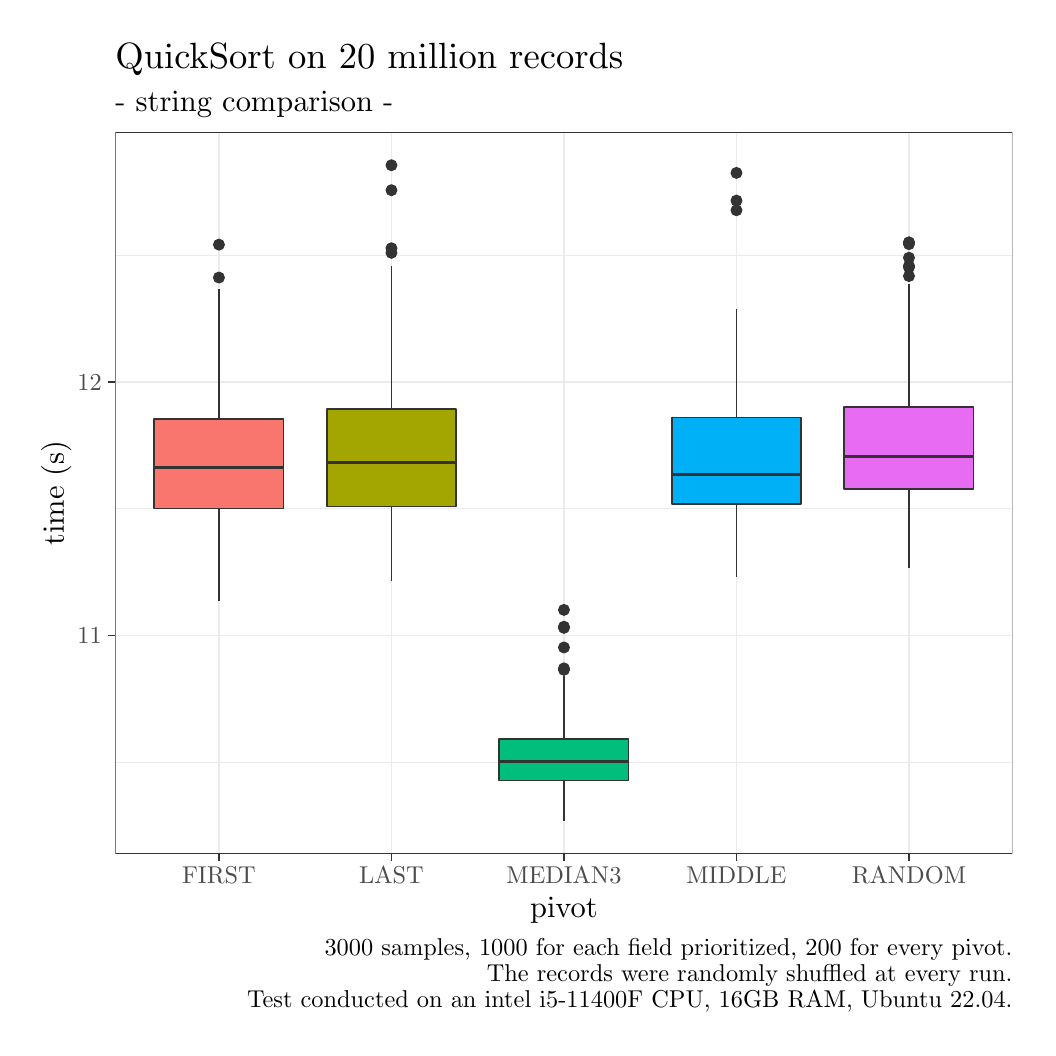
\begin{tikzpicture}[x=1pt,y=1pt]
\definecolor{fillColor}{RGB}{255,255,255}
\path[use as bounding box,fill=fillColor,fill opacity=0.00] (0,0) rectangle (361.35,361.35);
\begin{scope}
\path[clip] (  0.00,  0.00) rectangle (361.35,361.35);
\definecolor{drawColor}{RGB}{255,255,255}
\definecolor{fillColor}{RGB}{255,255,255}

\path[draw=drawColor,line width= 0.6pt,line join=round,line cap=round,fill=fillColor] (  0.00,  0.00) rectangle (361.35,361.35);
\end{scope}
\begin{scope}
\path[clip] ( 31.71, 62.97) rectangle (355.85,323.48);
\definecolor{fillColor}{RGB}{255,255,255}

\path[fill=fillColor] ( 31.71, 62.97) rectangle (355.85,323.48);
\definecolor{drawColor}{gray}{0.92}

\path[draw=drawColor,line width= 0.3pt,line join=round] ( 31.71, 95.88) --
	(355.85, 95.88);

\path[draw=drawColor,line width= 0.3pt,line join=round] ( 31.71,187.53) --
	(355.85,187.53);

\path[draw=drawColor,line width= 0.3pt,line join=round] ( 31.71,279.19) --
	(355.85,279.19);

\path[draw=drawColor,line width= 0.6pt,line join=round] ( 31.71,141.71) --
	(355.85,141.71);

\path[draw=drawColor,line width= 0.6pt,line join=round] ( 31.71,233.36) --
	(355.85,233.36);

\path[draw=drawColor,line width= 0.6pt,line join=round] ( 69.11, 62.97) --
	( 69.11,323.48);

\path[draw=drawColor,line width= 0.6pt,line join=round] (131.45, 62.97) --
	(131.45,323.48);

\path[draw=drawColor,line width= 0.6pt,line join=round] (193.78, 62.97) --
	(193.78,323.48);

\path[draw=drawColor,line width= 0.6pt,line join=round] (256.12, 62.97) --
	(256.12,323.48);

\path[draw=drawColor,line width= 0.6pt,line join=round] (318.45, 62.97) --
	(318.45,323.48);
\definecolor{drawColor}{gray}{0.20}
\definecolor{fillColor}{gray}{0.20}

\path[draw=drawColor,line width= 0.4pt,line join=round,line cap=round,fill=fillColor] ( 69.11,282.95) circle (  1.96);

\path[draw=drawColor,line width= 0.4pt,line join=round,line cap=round,fill=fillColor] ( 69.11,271.05) circle (  1.96);

\path[draw=drawColor,line width= 0.6pt,line join=round] ( 69.11,219.87) -- ( 69.11,266.89);

\path[draw=drawColor,line width= 0.6pt,line join=round] ( 69.11,187.58) -- ( 69.11,154.24);
\definecolor{fillColor}{RGB}{248,118,109}

\path[draw=drawColor,line width= 0.6pt,line join=round,line cap=round,fill=fillColor] ( 45.74,219.87) --
	( 45.74,187.58) --
	( 92.49,187.58) --
	( 92.49,219.87) --
	( 45.74,219.87) --
	cycle;

\path[draw=drawColor,line width= 1.1pt,line join=round] ( 45.74,202.45) -- ( 92.49,202.45);
\definecolor{fillColor}{gray}{0.20}

\path[draw=drawColor,line width= 0.4pt,line join=round,line cap=round,fill=fillColor] (131.45,302.62) circle (  1.96);

\path[draw=drawColor,line width= 0.4pt,line join=round,line cap=round,fill=fillColor] (131.45,279.99) circle (  1.96);

\path[draw=drawColor,line width= 0.4pt,line join=round,line cap=round,fill=fillColor] (131.45,281.65) circle (  1.96);

\path[draw=drawColor,line width= 0.4pt,line join=round,line cap=round,fill=fillColor] (131.45,311.64) circle (  1.96);

\path[draw=drawColor,line width= 0.6pt,line join=round] (131.45,223.49) -- (131.45,275.29);

\path[draw=drawColor,line width= 0.6pt,line join=round] (131.45,188.32) -- (131.45,161.50);
\definecolor{fillColor}{RGB}{163,165,0}

\path[draw=drawColor,line width= 0.6pt,line join=round,line cap=round,fill=fillColor] (108.07,223.49) --
	(108.07,188.32) --
	(154.82,188.32) --
	(154.82,223.49) --
	(108.07,223.49) --
	cycle;

\path[draw=drawColor,line width= 1.1pt,line join=round] (108.07,204.32) -- (154.82,204.32);
\definecolor{fillColor}{gray}{0.20}

\path[draw=drawColor,line width= 0.4pt,line join=round,line cap=round,fill=fillColor] (193.78,144.48) circle (  1.96);

\path[draw=drawColor,line width= 0.4pt,line join=round,line cap=round,fill=fillColor] (193.78,129.31) circle (  1.96);

\path[draw=drawColor,line width= 0.4pt,line join=round,line cap=round,fill=fillColor] (193.78,150.96) circle (  1.96);

\path[draw=drawColor,line width= 0.4pt,line join=round,line cap=round,fill=fillColor] (193.78,144.89) circle (  1.96);

\path[draw=drawColor,line width= 0.4pt,line join=round,line cap=round,fill=fillColor] (193.78,137.39) circle (  1.96);

\path[draw=drawColor,line width= 0.4pt,line join=round,line cap=round,fill=fillColor] (193.78,129.82) circle (  1.96);

\path[draw=drawColor,line width= 0.6pt,line join=round] (193.78,104.38) -- (193.78,126.91);

\path[draw=drawColor,line width= 0.6pt,line join=round] (193.78, 89.28) -- (193.78, 74.81);
\definecolor{fillColor}{RGB}{0,191,125}

\path[draw=drawColor,line width= 0.6pt,line join=round,line cap=round,fill=fillColor] (170.41,104.38) --
	(170.41, 89.28) --
	(217.16, 89.28) --
	(217.16,104.38) --
	(170.41,104.38) --
	cycle;

\path[draw=drawColor,line width= 1.1pt,line join=round] (170.41, 96.28) -- (217.16, 96.28);
\definecolor{fillColor}{gray}{0.20}

\path[draw=drawColor,line width= 0.4pt,line join=round,line cap=round,fill=fillColor] (256.12,308.87) circle (  1.96);

\path[draw=drawColor,line width= 0.4pt,line join=round,line cap=round,fill=fillColor] (256.12,295.37) circle (  1.96);

\path[draw=drawColor,line width= 0.4pt,line join=round,line cap=round,fill=fillColor] (256.12,298.86) circle (  1.96);

\path[draw=drawColor,line width= 0.6pt,line join=round] (256.12,220.43) -- (256.12,259.67);

\path[draw=drawColor,line width= 0.6pt,line join=round] (256.12,189.29) -- (256.12,162.96);
\definecolor{fillColor}{RGB}{0,176,246}

\path[draw=drawColor,line width= 0.6pt,line join=round,line cap=round,fill=fillColor] (232.74,220.43) --
	(232.74,189.29) --
	(279.49,189.29) --
	(279.49,220.43) --
	(232.74,220.43) --
	cycle;

\path[draw=drawColor,line width= 1.1pt,line join=round] (232.74,200.05) -- (279.49,200.05);
\definecolor{fillColor}{gray}{0.20}

\path[draw=drawColor,line width= 0.4pt,line join=round,line cap=round,fill=fillColor] (318.45,283.70) circle (  1.96);

\path[draw=drawColor,line width= 0.4pt,line join=round,line cap=round,fill=fillColor] (318.45,283.76) circle (  1.96);

\path[draw=drawColor,line width= 0.4pt,line join=round,line cap=round,fill=fillColor] (318.45,278.22) circle (  1.96);

\path[draw=drawColor,line width= 0.4pt,line join=round,line cap=round,fill=fillColor] (318.45,275.31) circle (  1.96);

\path[draw=drawColor,line width= 0.4pt,line join=round,line cap=round,fill=fillColor] (318.45,271.59) circle (  1.96);

\path[draw=drawColor,line width= 0.4pt,line join=round,line cap=round,fill=fillColor] (318.45,274.74) circle (  1.96);

\path[draw=drawColor,line width= 0.4pt,line join=round,line cap=round,fill=fillColor] (318.45,283.12) circle (  1.96);

\path[draw=drawColor,line width= 0.6pt,line join=round] (318.45,224.37) -- (318.45,268.72);

\path[draw=drawColor,line width= 0.6pt,line join=round] (318.45,194.56) -- (318.45,166.20);
\definecolor{fillColor}{RGB}{231,107,243}

\path[draw=drawColor,line width= 0.6pt,line join=round,line cap=round,fill=fillColor] (295.07,224.37) --
	(295.07,194.56) --
	(341.82,194.56) --
	(341.82,224.37) --
	(295.07,224.37) --
	cycle;

\path[draw=drawColor,line width= 1.1pt,line join=round] (295.07,206.25) -- (341.82,206.25);

\path[draw=drawColor,line width= 0.6pt,line join=round,line cap=round] ( 31.71, 62.97) rectangle (355.85,323.48);
\end{scope}
\begin{scope}
\path[clip] (  0.00,  0.00) rectangle (361.35,361.35);
\definecolor{drawColor}{gray}{0.30}

\node[text=drawColor,anchor=base east,inner sep=0pt, outer sep=0pt, scale=  0.88] at ( 26.76,138.68) {11};

\node[text=drawColor,anchor=base east,inner sep=0pt, outer sep=0pt, scale=  0.88] at ( 26.76,230.33) {12};
\end{scope}
\begin{scope}
\path[clip] (  0.00,  0.00) rectangle (361.35,361.35);
\definecolor{drawColor}{gray}{0.20}

\path[draw=drawColor,line width= 0.6pt,line join=round] ( 28.96,141.71) --
	( 31.71,141.71);

\path[draw=drawColor,line width= 0.6pt,line join=round] ( 28.96,233.36) --
	( 31.71,233.36);
\end{scope}
\begin{scope}
\path[clip] (  0.00,  0.00) rectangle (361.35,361.35);
\definecolor{drawColor}{gray}{0.20}

\path[draw=drawColor,line width= 0.6pt,line join=round] ( 69.11, 60.22) --
	( 69.11, 62.97);

\path[draw=drawColor,line width= 0.6pt,line join=round] (131.45, 60.22) --
	(131.45, 62.97);

\path[draw=drawColor,line width= 0.6pt,line join=round] (193.78, 60.22) --
	(193.78, 62.97);

\path[draw=drawColor,line width= 0.6pt,line join=round] (256.12, 60.22) --
	(256.12, 62.97);

\path[draw=drawColor,line width= 0.6pt,line join=round] (318.45, 60.22) --
	(318.45, 62.97);
\end{scope}
\begin{scope}
\path[clip] (  0.00,  0.00) rectangle (361.35,361.35);
\definecolor{drawColor}{gray}{0.30}

\node[text=drawColor,anchor=base,inner sep=0pt, outer sep=0pt, scale=  0.88] at ( 69.11, 51.95) {FIRST};

\node[text=drawColor,anchor=base,inner sep=0pt, outer sep=0pt, scale=  0.88] at (131.45, 51.95) {LAST};

\node[text=drawColor,anchor=base,inner sep=0pt, outer sep=0pt, scale=  0.88] at (193.78, 51.95) {MEDIAN3};

\node[text=drawColor,anchor=base,inner sep=0pt, outer sep=0pt, scale=  0.88] at (256.12, 51.95) {MIDDLE};

\node[text=drawColor,anchor=base,inner sep=0pt, outer sep=0pt, scale=  0.88] at (318.45, 51.95) {RANDOM};
\end{scope}
\begin{scope}
\path[clip] (  0.00,  0.00) rectangle (361.35,361.35);
\definecolor{drawColor}{RGB}{0,0,0}

\node[text=drawColor,anchor=base,inner sep=0pt, outer sep=0pt, scale=  1.10] at (193.78, 39.92) {pivot};
\end{scope}
\begin{scope}
\path[clip] (  0.00,  0.00) rectangle (361.35,361.35);
\definecolor{drawColor}{RGB}{0,0,0}

\node[text=drawColor,rotate= 90.00,anchor=base,inner sep=0pt, outer sep=0pt, scale=  1.10] at ( 13.08,193.22) {time (s)};
\end{scope}
\begin{scope}
\path[clip] (  0.00,  0.00) rectangle (361.35,361.35);
\definecolor{drawColor}{RGB}{0,0,0}

\node[text=drawColor,anchor=base west,inner sep=0pt, outer sep=0pt, scale=  1.10] at ( 31.71,331.12) {- string comparison -};
\end{scope}
\begin{scope}
\path[clip] (  0.00,  0.00) rectangle (361.35,361.35);
\definecolor{drawColor}{RGB}{0,0,0}

\node[text=drawColor,anchor=base west,inner sep=0pt, outer sep=0pt, scale=  1.32] at ( 31.71,346.76) {QuickSort on 20 million records};
\end{scope}
\begin{scope}
\path[clip] (  0.00,  0.00) rectangle (361.35,361.35);
\definecolor{drawColor}{RGB}{0,0,0}

\node[text=drawColor,anchor=base east,inner sep=0pt, outer sep=0pt, scale=  0.88] at (355.85, 26.22) {3000 samples, 1000 for each field prioritized, 200 for every pivot.};

\node[text=drawColor,anchor=base east,inner sep=0pt, outer sep=0pt, scale=  0.88] at (355.85, 16.71) {                       The records were randomly shuffled at every run.};

\node[text=drawColor,anchor=base east,inner sep=0pt, outer sep=0pt, scale=  0.88] at (355.85,  7.21) {                       Test conducted on an intel i5-11400F CPU, 16GB RAM, Ubuntu 22.04.};
\end{scope}
\end{tikzpicture}
